\documentclass{article}
\usepackage{tikz}
\usetikzlibrary{intersections}
\usepackage{xcolor}

\begin{document}
    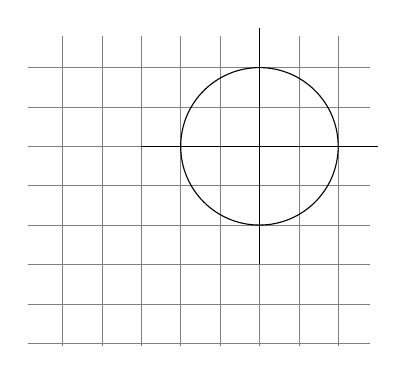
\begin{tikzpicture}
        \draw[step=.5cm, gray, very thin] (-1.4, -1,4) grid (1.4, 1.4);
        \draw (-1.5, 0) -- (1.5, 0);
        \draw (0, -1.5) -- (0, 1.5);
        \draw (0, 0) circle[radius=1cm];
    \end{tikzpicture}
    \newpage
    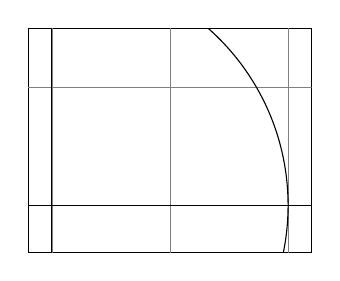
\begin{tikzpicture}[scale=3]
        \clip[draw] (-0.1, -0.2) rectangle (1.1, 0.75);
        \draw[step=.5cm, gray, very thin] (-1.4, -1,4) grid (1.4, 1.4);
        \draw (-1.5, 0) -- (1.5, 0);
        \draw (0, -1.5) -- (0, 1.5);
        \draw (0, 0) circle[radius=1cm];
    \end{tikzpicture}
    \newpage
    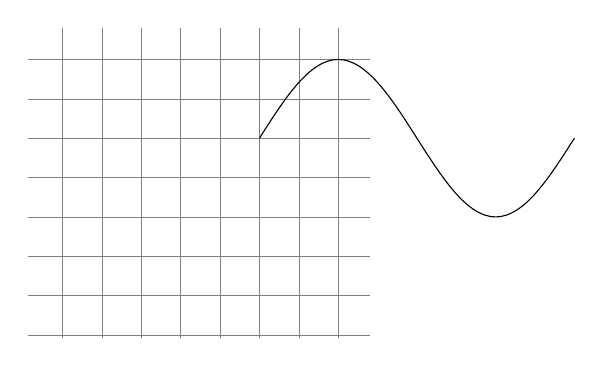
\begin{tikzpicture}
        \draw[step=.5cm, gray, very thin] (-1.4, -1,4) grid (1.4, 1.4);
        \draw (0, 0) sin (1, 1) cos (2, 0) sin (3, -1) cos (4, 0);
    \end{tikzpicture}
    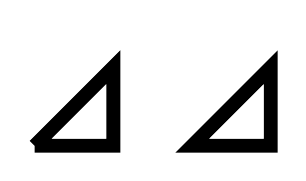
\begin{tikzpicture}[line width=5pt]
        \draw (0,0) -- (1,0) -- (1,1) -- (0,0);
        \draw (2,0) -- (3,0) -- (3,1) -- cycle;
        \useasboundingbox (0,1.5);
    \end{tikzpicture}
    \newline
    
\begin{tikzpicture}[rounded corners,ultra thick]
        \shade[top color=yellow,bottom color=black] (0,0) rectangle +(2,1);
        \shade[left color=yellow,right color=black] (3,0) rectangle +(2,1);
        \shadedraw[inner color=yellow,outer color=black,draw=red] (6,0) rectangle +(2,1);
        \shade[ball color=green] (9,.5) circle (.5cm);
    \end{tikzpicture}
    \newline
    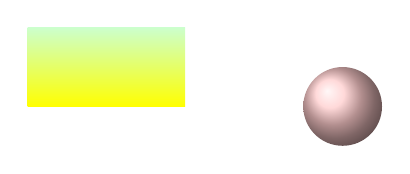
\begin{tikzpicture}
        \shade[top color=green!20!white, bottom color=yellow] (0, 0) rectangle +(2, 1);
        \shade[ball color=red!20!white] (4, 0) circle (.5cm);
    \end{tikzpicture}
    \newpage
    How about the difference between + and ++?
    \newline
    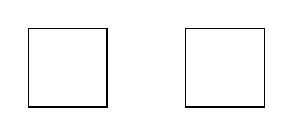
\begin{tikzpicture}
        \def\rectanglepath{-- ++(1cm, 0) -- ++(0, 1cm) -- ++(-1cm, 0) -- cycle}
        \draw (0, 0) \rectanglepath;
        \draw (2, 0) \rectanglepath;
    \end{tikzpicture}
    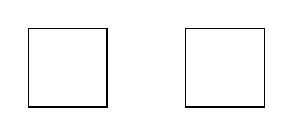
\begin{tikzpicture}
        \def\rectanglePath{-- +(1cm, 0) -- +(1cm, 1cm) -- +(0, 1cm) -- cycle}
        \draw (0, 0) \rectanglePath;
        \draw (2, 0) \rectanglePath;
    \end{tikzpicture}
    \newline
    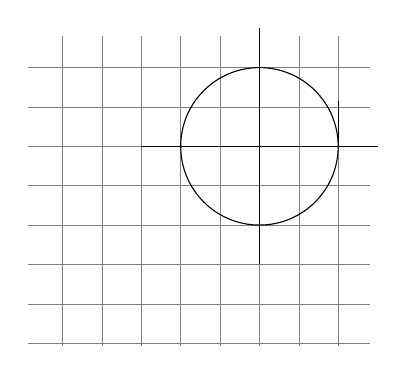
\begin{tikzpicture}
        % \clip[draw] (-0.1, -0.2) rectangle (1.1, 0.75);
        \draw[step=.5cm, gray, very thin] (-1.4, -1,4) grid (1.4, 1.4);
        \draw (-1.5, 0) -- (1.5, 0);
        \draw (0, -1.5) -- (0, 1.5);
        \draw (0, 0) circle[radius=1cm];
        \path[name path=upward line] (1, 0) -- (1, 1);
        \path[name path=sloped line] (0, 0) -- (30:1.5cm);
        \draw[name intersections={of=upward line and sloped line, by=x}] (1, 0) -- (x);
    \end{tikzpicture}
\end{document}